\chapter{Taylor Expansions, Asymptotic Developments \& Riemann Integration}
\label{chap:taylor_integrals}

\section{Higher-Order Derivatives and Leibniz's Formula}

Let $f: I \longrightarrow \mathbb{R}$ be an $n$-times differentiable function on an interval $I$. The successive derivatives are defined recursively by $f^{(0)} = f$, $f^{(1)} = f'$, and $f^{(k+1)} = (f^{(k)})'$. If $f^{(n)}$ is continuous on $I$, we write $f \in \mathcal{C}^n(I)$. If $f$ is infinitely differentiable, $f \in \mathcal{C}^\infty(I)$.

\begin{figure}[htbp]
  \centering
  \begin{minipage}{0.30\textwidth}
    \centering
    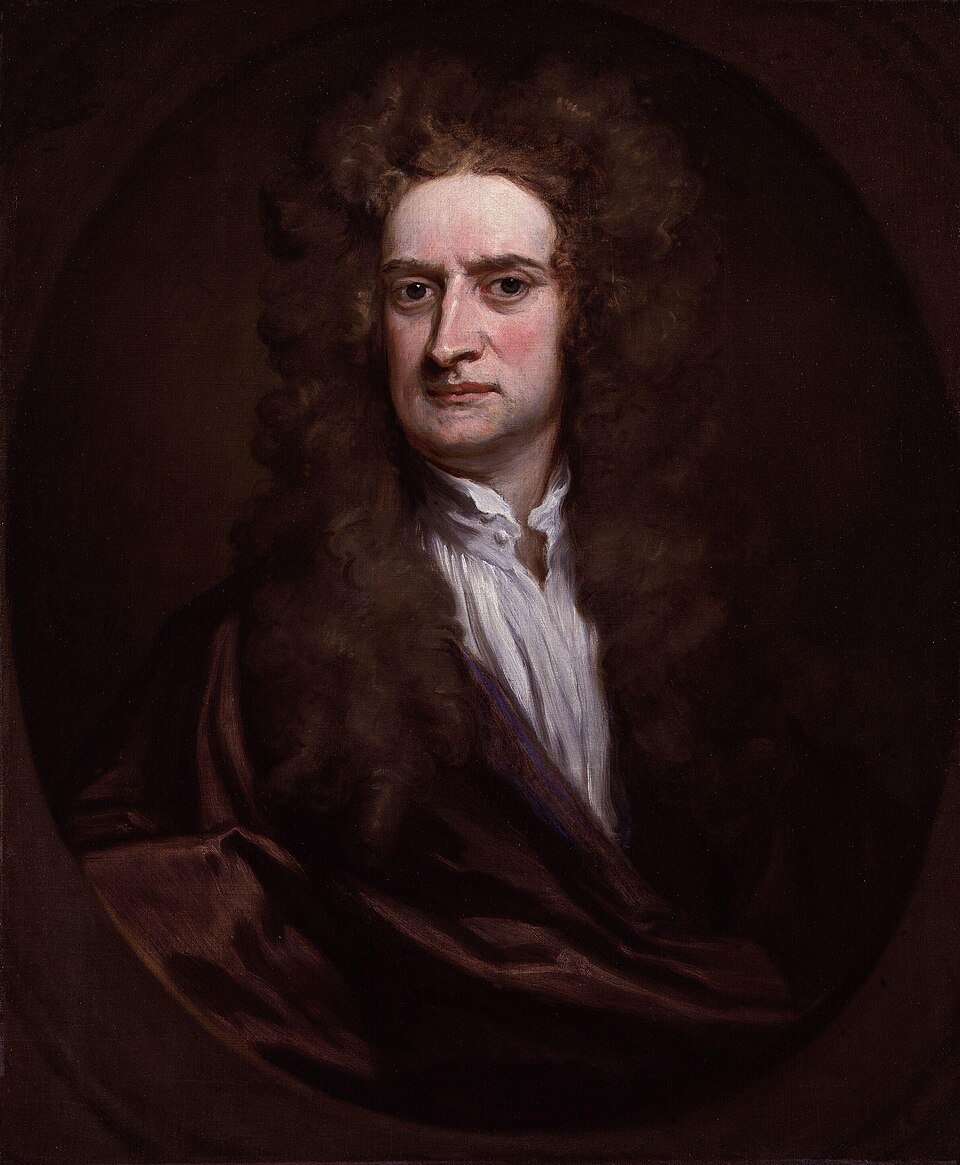
\includegraphics[width=0.88\textwidth]{newton.jpg}
    \caption*{(a) \textbf{Isaac Newton (1642--1727)}}
  \end{minipage}
  \hfill
  \begin{minipage}{0.30\textwidth}
    \centering
    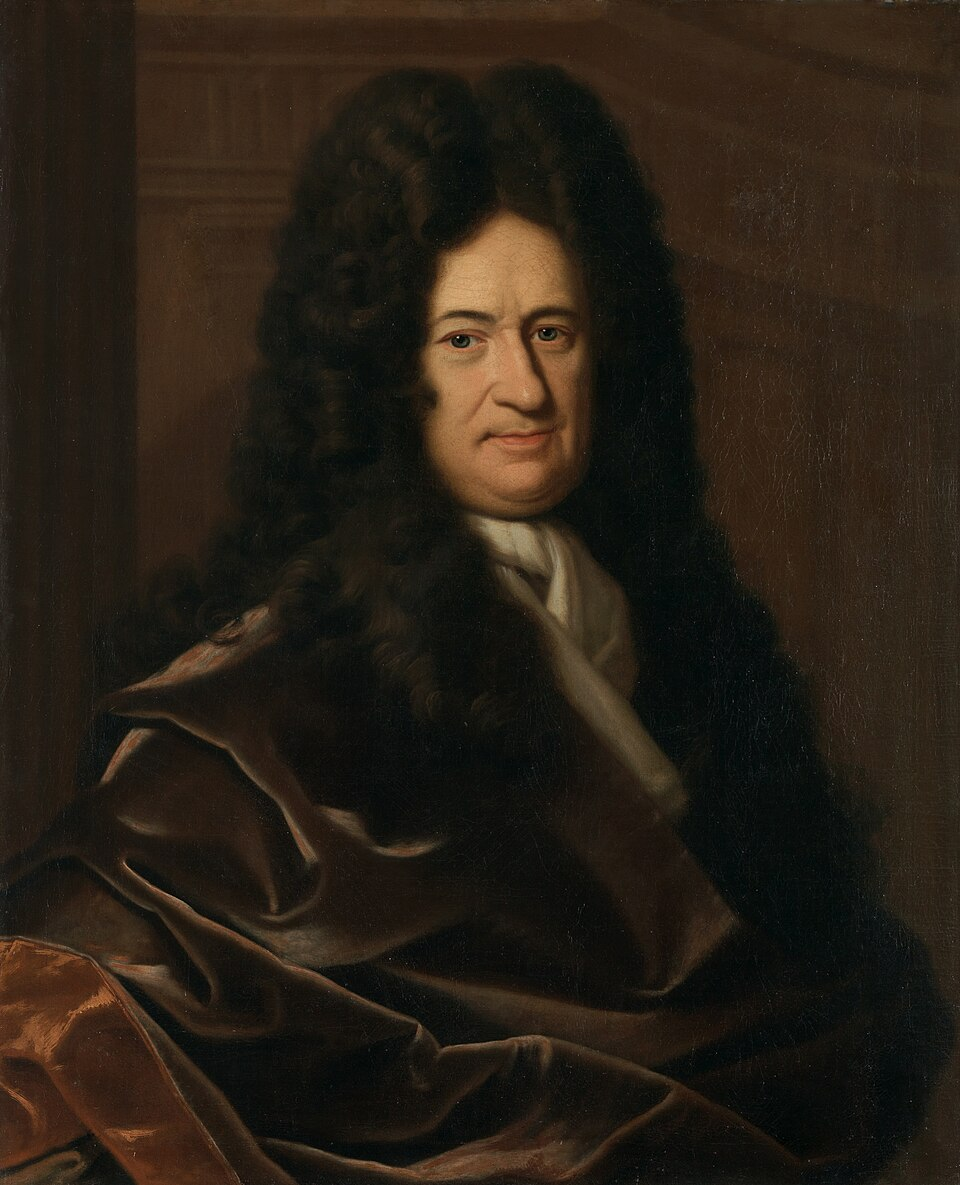
\includegraphics[width=0.88\textwidth]{leibniz.jpg}
    \caption*{(b) \textbf{Gottfried Leibniz (1646--1716)}}
  \end{minipage}
  \hfill
  \begin{minipage}{0.30\textwidth}
    \centering
    
\includegraphics[width=0.88\textwidth]{taylor.jpg}
    \caption*{(c) \textbf{Brook Taylor (1685--1731)}}
  \end{minipage}
  \caption{\textbf{Architects of the Infinitesimal Calculus:} Sir Isaac Newton (fluxions and physics foundations), Gottfried Wilhelm Leibniz (differential and integral notation $\dd x, \int$), and Brook Taylor (originator of Taylor polynomial expansions in 1715).}
  \label{fig:calculus_founders}
\end{figure}

\begin{theorembox}{Leibniz's Formula for Product Differentiation}
Let $u, v: I \longrightarrow \mathbb{R}$ be two functions of class $\mathcal{C}^n(I)$.
The $n$-th derivative of their product $u \cdot v$ is given by the binomial convolution:
\begin{equation}
(u \cdot v)^{(n)}(x) = \sum_{k=0}^n \binom{n}{k} u^{(k)}(x) \cdot v^{(n-k)}(x), \qquad \text{where } \binom{n}{k} = \frac{n!}{k!(n-k)!}.
\end{equation}
\end{theorembox}

\section{Taylor's Theorems: Lagrange and Peano (Young) Remainders}

\begin{theorembox}{Taylor's Theorem with Lagrange Remainder}
Let $f \in \mathcal{C}^n([a, b])$ such that $f^{(n+1)}$ exists on the open interval $(a, b)$.
For any $x_0, x \in [a, b]$, there exists at least one real number $c$ strictly between $x_0$ and $x$ such that:
\begin{equation}
f(x) = \sum_{k=0}^n \frac{f^{(k)}(x_0)}{k!} (x - x_0)^k + \frac{f^{(n+1)}(c)}{(n+1)!} (x - x_0)^{n+1}.
\end{equation}
The polynomial $P_n(x) = \sum_{k=0}^n \frac{f^{(k)}(x_0)}{k!} (x - x_0)^k$ is the **$n$-th Taylor polynomial**, and $R_n(x) = \frac{f^{(n+1)}(c)}{(n+1)!} (x - x_0)^{n+1}$ is the **Lagrange remainder**.
\end{theorembox}

\begin{figure}[htbp]
  \centering
  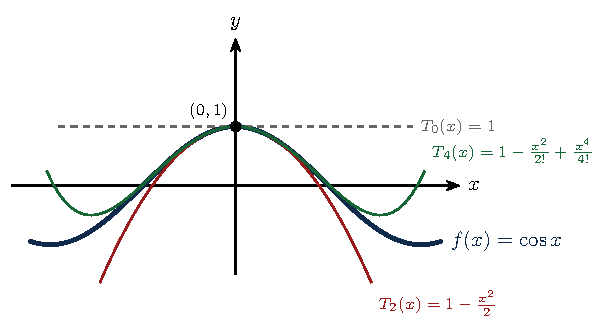
\includegraphics[width=0.88\textwidth]{07_taylor_polynomials.pdf}
  \caption{\textbf{Taylor Polynomial Approximations of $\cos x$ at $x_0 = 0$:} The zero-order polynomial $T_0(x) = 1$, second-order parabola $T_2(x) = 1 - \frac{x^2}{2}$, and fourth-order polynomial $T_4(x) = 1 - \frac{x^2}{2!} + \frac{x^4}{4!}$ progressively hug the true cosine curve over wider domains.}
  \label{fig:taylor_plots}
\end{figure}

\begin{theorembox}{Taylor-Young Formula (Local Expansion with Peano Remainder)}
If $f$ is $n$-times differentiable at $x_0$, then as $x \to x_0$:
\begin{equation}
f(x) = \sum_{k=0}^n \frac{f^{(k)}(x_0)}{k!} (x - x_0)^k + o\big((x - x_0)^n\big) \quad \text{as } x \to x_0,
\end{equation}
where $o\big((x - x_0)^n\big) = (x - x_0)^n \varepsilon(x)$ with $\lim_{x \to x_0} \varepsilon(x) = 0$ (Landau's small-$o$ notation).
\end{theorembox}

\section{Limited Developments (Développements Limités at $0$)}

\begin{definitionbox}{Limited Development of Order $n$ at $0$ ($\mathrm{DL}_n(0)$)}
A function $f$ admits a \textbf{limited development} of order $n \in \mathbb{N}$ in the neighborhood of $0$ if there exists a polynomial $P_n(x) = a_0 + a_1 x + a_2 x^2 + \dots + a_n x^n$ of degree $\le n$ such that:
\begin{equation}
f(x) = P_n(x) + x^n \varepsilon(x) \quad \text{with} \quad \lim_{x \to 0} \varepsilon(x) = 0.
\end{equation}
The polynomial $P_n(x)$ is \textbf{strictly unique}. If $f$ is $n$-times differentiable, $a_k = \frac{f^{(k)}(0)}{k!}$ (Maclaurin expansion).
\end{definitionbox}

\begin{propbox}{Reference Maclaurin Expansions at $x = 0$}
As $x \to 0$, the following standard limited developments hold:
\begin{align}
e^x &= 1 + x + \frac{x^2}{2!} + \frac{x^3}{3!} + \dots + \frac{x^n}{n!} + o(x^n) \\
\sin x &= x - \frac{x^3}{3!} + \frac{x^5}{5!} - \dots + (-1)^p \frac{x^{2p+1}}{(2p+1)!} + o(x^{2p+2}) \\
\cos x &= 1 - \frac{x^2}{2!} + \frac{x^4}{4!} - \dots + (-1)^p \frac{x^{2p}}{(2p)!} + o(x^{2p+1}) \\
\ln(1 + x) &= x - \frac{x^2}{2} + \frac{x^3}{3} - \frac{x^4}{4} + \dots + (-1)^{n-1} \frac{x^n}{n} + o(x^n) \\
(1 + x)^\alpha &= 1 + \alpha x + \frac{\alpha(\alpha-1)}{2!} x^2 + \dots + \frac{\alpha(\alpha-1)\cdots(\alpha-n+1)}{n!} x^n + o(x^n) \\
\frac{1}{1 - x} &= 1 + x + x^2 + x^3 + \dots + x^n + o(x^n) \\
\frac{1}{1 + x} &= 1 - x + x^2 - x^3 + \dots + (-1)^n x^n + o(x^n) \\
\arctan x &= x - \frac{x^3}{3} + \frac{x^5}{5} - \dots + (-1)^p \frac{x^{2p+1}}{2p+1} + o(x^{2p+2})
\end{align}
\end{propbox}

\section{The Riemann Integral and Fundamental Theorem of Calculus}

\begin{figure}[htbp]
  \centering
  \begin{minipage}{0.35\textwidth}
    \centering
    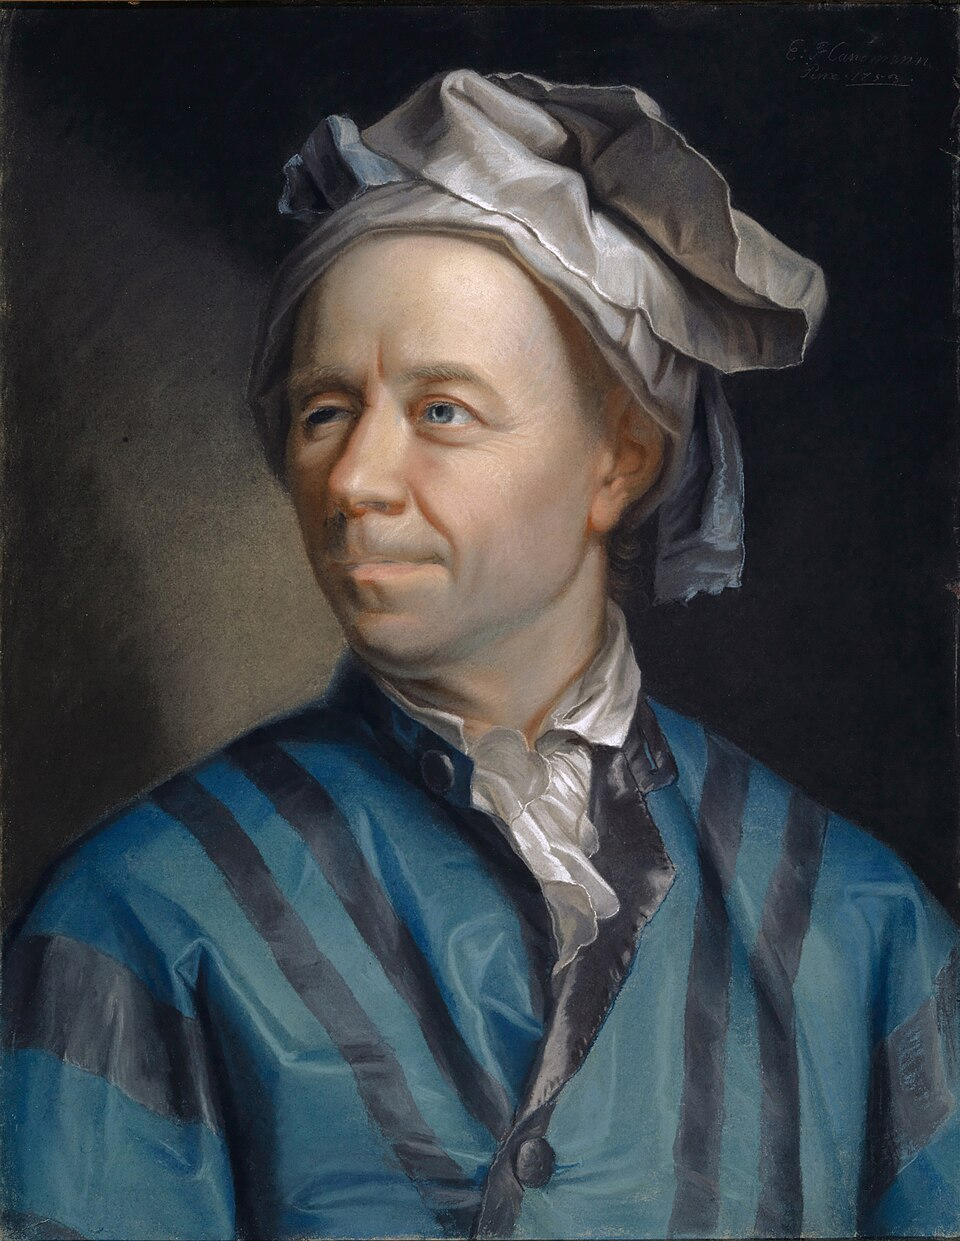
\includegraphics[width=0.82\textwidth]{euler.jpg}
    \caption*{(a) \textbf{Leonhard Euler (1707--1783)}}
  \end{minipage}
  \hspace{0.08\textwidth}
  \begin{minipage}{0.35\textwidth}
    \centering
    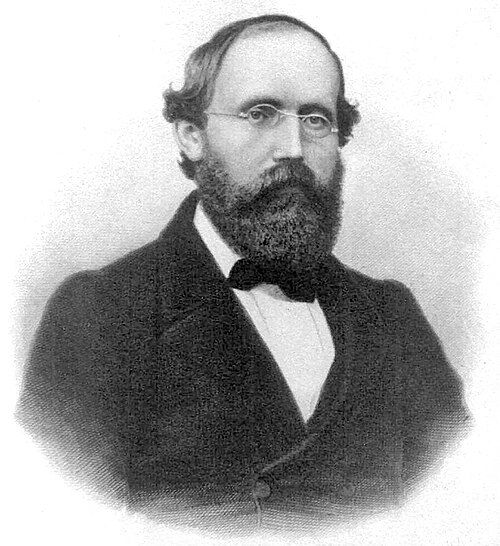
\includegraphics[width=0.82\textwidth]{riemann.jpg}
    \caption*{(b) \textbf{Bernhard Riemann (1826--1866)}}
  \end{minipage}
  \caption{\textbf{Pioneers of Integral Analysis:} Leonhard Euler (master of analytical transformations and infinite sums) and Bernhard Riemann (creator of the modern definition of the definite integral via partition step sums).}
  \label{fig:euler_riemann}
\end{figure}

\begin{definitionbox}{The Riemann Integral}
Let $f: [a, b] \longrightarrow \mathbb{R}$ be a bounded function.
A \textbf{subdivision} (partition) of $[a, b]$ is a finite ordered sequence $\sigma = \{a = x_0 < x_1 < x_2 < \dots < x_n = b\}$.
For any choice of evaluation tags $\xi_i \in [x_{i-1}, x_i]$, the \textbf{Riemann sum} is:
\begin{equation}
S(f, \sigma, \xi) = \sum_{i=1}^n f(\xi_i) \cdot (x_i - x_{i-1}) = \sum_{i=1}^n f(\xi_i) \Delta x_i.
\end{equation}
$f$ is \textbf{Riemann integrable} on $[a, b]$ if the Riemann sums converge to a unique real limit as the mesh size $\max_i \Delta x_i \to 0$:
\begin{equation}
\int_a^b f(x)\,\dd x = \lim_{\|\sigma\| \to 0} \sum_{i=1}^n f(\xi_i) \Delta x_i.
\end{equation}
\textbf{Integrability Criterion:} Every continuous function on $[a, b]$ ($f \in \mathcal{C}^0([a, b])$) and every piecewise continuous monotonic function is Riemann integrable.
\end{definitionbox}

\begin{figure}[htbp]
  \centering
  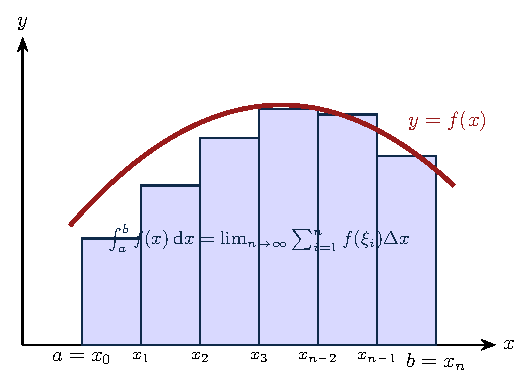
\includegraphics[width=0.88\textwidth]{08_riemann_integral.pdf}
  \caption{\textbf{Riemann Integral as the Limit of Rectangular Approximations:} Subdividing $[a, b]$ into $n$ subintervals and summing the areas of rectangular slices converges to the exact geometric area under $y = f(x)$.}
  \label{fig:riemann_rectangles}
\end{figure}

\begin{theorembox}{The Fundamental Theorem of Calculus (FTC)}
\begin{enumerate}[leftmargin=1.4em,itemsep=3pt]
  \item \textbf{First Part (Existence of Antiderivatives):}
  Let $f: [a, b] \longrightarrow \mathbb{R}$ be continuous. The function $F: [a, b] \longrightarrow \mathbb{R}$ defined by:
  \[
  F(x) = \int_a^x f(t)\,\dd t
  \]
  is continuous on $[a, b]$, differentiable on $(a, b)$, and its derivative is identically $f$:
  \[
  F'(x) = \frac{\dd}{\dd x} \left( \int_a^x f(t)\,\dd t \right) = f(x) \quad \text{for all } x \in [a, b].
  \]
  \item \textbf{Second Part (Newton-Leibniz Formula):}
  If $G$ is any antiderivative of $f$ on $[a, b]$ (so $G'(x) = f(x)$):
  \begin{equation}
  \int_a^b f(t)\,\dd t = G(b) - G(a) = \big[ G(t) \big]_a^b.
  \end{equation}
\end{enumerate}
\end{theorembox}

\begin{propbox}{Essential Integration Techniques}
\begin{enumerate}[leftmargin=1.4em,itemsep=3pt]
  \item \textbf{Integration by Parts (IPP):}
  Let $u, v \in \mathcal{C}^1([a, b])$:
  \begin{equation}
  \int_a^b u(t) v'(t)\,\dd t = \big[ u(t) v(t) \big]_a^b - \int_a^b u'(t) v(t)\,\dd t.
  \end{equation}
  \item \textbf{Integration by Substitution (Change of Variable):}
  Let $\phi: [\alpha, \beta] \longrightarrow [a, b]$ be a function of class $\mathcal{C}^1$ with $\phi(\alpha) = a$ and $\phi(\beta) = b$, and let $f \in \mathcal{C}^0([a, b])$:
  \begin{equation}
  \int_a^b f(x)\,\dd x = \int_\alpha^\beta f(\phi(t)) \cdot \phi'(t)\,\dd t.
  \end{equation}
\end{enumerate}
\end{propbox}

\section{Worked Examples with Step-by-Step Proofs}

\begin{workedexample}{High-Order Derivative Using Leibniz's Product Rule}
Compute the $n$-th derivative of the function:
\[
f(x) = x^2 e^{3x}.
\]

\paragraph{Solution and Proof.}
Write $f(x) = u(x) \cdot v(x)$ where:
\[
u(x) = x^2, \qquad v(x) = e^{3x}.
\]
Compute the successive derivatives of $u(x)$:
\[
u^{(0)}(x) = x^2, \quad u^{(1)}(x) = 2x, \quad u^{(2)}(x) = 2, \quad \text{and} \quad u^{(k)}(x) = 0 \quad \text{for all } k \ge 3.
\]
Compute the successive derivatives of $v(x)$:
\[
v^{(k)}(x) = 3^k e^{3x} \quad \text{for all } k \ge 0.
\]
Applying **Leibniz's Formula**:
\[
f^{(n)}(x) = \sum_{k=0}^n \binom{n}{k} u^{(k)}(x) v^{(n-k)}(x).
\]
Since $u^{(k)}(x) = 0$ for all $k \ge 3$, only the first three terms ($k = 0, 1, 2$) survive:
\begin{align*}
f^{(n)}(x) &= \binom{n}{0} u(x) v^{(n)}(x) + \binom{n}{1} u'(x) v^{(n-1)}(x) + \binom{n}{2} u''(x) v^{(n-2)}(x) \\
           &= 1 \cdot (x^2) \cdot \left( 3^n e^{3x} \right) + n \cdot (2x) \cdot \left( 3^{n-1} e^{3x} \right) + \frac{n(n-1)}{2} \cdot (2) \cdot \left( 3^{n-2} e^{3x} \right).
\end{align*}
Factor out the common exponential and power term $3^{n-2} e^{3x}$:
\begin{align*}
f^{(n)}(x) &= 3^{n-2} e^{3x} \left[ 3^2 x^2 + 2n \cdot 3 x + n(n-1) \right] \\
           &= \mathbf{3^{n-2} e^{3x} \left[ 9x^2 + 6nx + n(n-1) \right]}. \quad \blacksquare
\end{align*}
\end{workedexample}

\begin{workedexample}{Indeterminate Limit via Limited Development}
Compute using limited developments the limit:
\[
L = \lim_{x \to 0} \frac{\sin x - x \cos x}{x^3}.
\]

\paragraph{Solution and Proof.}
As $x \to 0$, the numerator approaches $\sin 0 - 0 = 0$ and the denominator $x^3 \to 0$, producing an indeterminate form of type $\left[ \frac{0}{0} \right]$.
Since the denominator is of degree $3$, we expand the numerator to order $3$ ($\mathrm{DL}_3(0)$).

Recall the reference Maclaurin expansions to order $3$:
\begin{align*}
\sin x &= x - \frac{x^3}{6} + o(x^3), \\
\cos x &= 1 - \frac{x^2}{2} + o(x^2).
\end{align*}
Multiply $\cos x$ by $x$:
\[
x \cos x = x \left( 1 - \frac{x^2}{2} + o(x^2) \right) = x - \frac{x^3}{2} + o(x^3).
\]
Subtract the two expressions:
\begin{align*}
\sin x - x \cos x &= \left( x - \frac{x^3}{6} + o(x^3) \right) - \left( x - \frac{x^3}{2} + o(x^3) \right) \\
                  &= (x - x) + \left( -\frac{1}{6} + \frac{1}{2} \right) x^3 + o(x^3) \\
                  &= \left( -\frac{1}{6} + \frac{3}{6} \right) x^3 + o(x^3) = \frac{2}{6} x^3 + o(x^3) = \frac{1}{3} x^3 + o(x^3).
\end{align*}
Now divide by the denominator $x^3$:
\[
\frac{\sin x - x \cos x}{x^3} = \frac{\frac{1}{3} x^3 + o(x^3)}{x^3} = \frac{1}{3} + \frac{o(x^3)}{x^3} = \frac{1}{3} + \varepsilon(x),
\]
where $\lim_{x \to 0} \varepsilon(x) = 0$.
Taking the limit as $x \to 0$:
\[
\mathbf{L = \lim_{x \to 0} \frac{\sin x - x \cos x}{x^3} = \frac{1}{3}}. \quad \blacksquare
\]
\end{workedexample}

\begin{workedexample}{Integration by Parts: Wallis Integrals}
Consider the sequence of \textbf{Wallis Integrals} defined for $n \in \mathbb{N}$ by:
\[
W_n = \int_0^{\pi/2} \sin^n(x)\,\dd x.
\]
\begin{enumerate}[leftmargin=1.4em,itemsep=2pt]
  \item Compute $W_0$ and $W_1$.
  \item Using integration by parts, establish the recurrence relation:
  \[
  W_n = \frac{n - 1}{n} W_{n-2} \quad \text{for all } n \ge 2.
  \]
\end{enumerate}

\paragraph{Solution and Proof.}
\textbf{1. Direct Evaluation of $W_0$ and $W_1$:}
\[
W_0 = \int_0^{\pi/2} 1\,\dd x = [x]_0^{\pi/2} = \mathbf{\frac{\pi}{2}}.
\]
\[
W_1 = \int_0^{\pi/2} \sin x\,\dd x = [-\cos x]_0^{\pi/2} = -\cos(\pi/2) - (-\cos 0) = 0 - (-1) = \mathbf{1}.
\]

\textbf{2. Integration by Parts for $n \ge 2$:}
Split the integrand: $\sin^n x = \sin^{n-1} x \cdot \sin x$.
Set:
\begin{align*}
u(x) &= \sin^{n-1} x \implies u'(x) = (n-1) \sin^{n-2} x \cos x, \\
v'(x) &= \sin x \implies v(x) = -\cos x.
\end{align*}
Applying the integration by parts formula:
\[
W_n = \big[ -\sin^{n-1}(x) \cos(x) \big]_0^{\pi/2} - \int_0^{\pi/2} (n-1) \sin^{n-2}(x) \cos(x) \cdot (-\cos x)\,\dd x.
\]
Evaluate the boundary bracket:
\begin{itemize}[itemsep=1pt]
  \item At $x = \pi/2$: $\cos(\pi/2) = 0$.
  \item At $x = 0$: for $n \ge 2$, $n - 1 \ge 1$, so $\sin^{n-1}(0) = 0$.
\end{itemize}
Thus the boundary term vanishes identically: $\big[ -\sin^{n-1}(x) \cos(x) \big]_0^{\pi/2} = 0$.
The integral term becomes:
\[
W_n = (n - 1) \int_0^{\pi/2} \sin^{n-2}(x) \cos^2(x)\,\dd x.
\]
Substitute the trigonometric identity $\cos^2 x = 1 - \sin^2 x$:
\begin{align*}
W_n &= (n - 1) \int_0^{\pi/2} \sin^{n-2}(x) (1 - \sin^2 x)\,\dd x \\
    &= (n - 1) \int_0^{\pi/2} \sin^{n-2}(x)\,\dd x - (n - 1) \int_0^{\pi/2} \sin^n(x)\,\dd x \\
    &= (n - 1) W_{n-2} - (n - 1) W_n.
\end{align*}
Rearranging terms in $W_n$:
\[
W_n + (n - 1) W_n = (n - 1) W_{n-2} \implies n W_n = (n - 1) W_{n-2}.
\]
Dividing across by $n > 0$:
\[
\mathbf{W_n = \frac{n - 1}{n} W_{n-2}}. \quad \blacksquare
\]
\end{workedexample}

\begin{workedexample}{Integration by Rational Substitution}
Compute the definite integral:
\[
I = \int_0^1 \frac{\dd x}{1 + \sqrt{x}}.
\]

\paragraph{Solution and Proof.}
The presence of the square root radical $\sqrt{x}$ suggests the change of variable:
\[
u = \sqrt{x} \iff x = u^2.
\]
Differentiating both sides:
\[
\dd x = 2u\,\dd u.
\]
Determine the new integration bounds:
\begin{itemize}[itemsep=1pt]
  \item When $x = 0$: $u = \sqrt{0} = 0$.
  \item When $x = 1$: $u = \sqrt{1} = 1$.
\end{itemize}
Substitute into the integral:
\[
I = \int_0^1 \frac{2u\,\dd u}{1 + u} = 2 \int_0^1 \frac{u}{u + 1}\,\dd u.
\]
Perform algebraic decomposition of the rational integrand by adding and subtracting $1$:
\[
\frac{u}{u + 1} = \frac{(u + 1) - 1}{u + 1} = 1 - \frac{1}{u + 1}.
\]
Now integrate term by term:
\begin{align*}
I &= 2 \int_0^1 \left( 1 - \frac{1}{u + 1} \right)\,\dd u = 2 \Big[ u - \ln(u + 1) \Big]_0^1 \\
  &= 2 \Big[ (1 - \ln 2) - (0 - \ln 1) \Big] \\
  &= 2(1 - \ln 2) = \mathbf{2 - 2 \ln 2} \approx \mathbf{0.6137}. \quad \blacksquare
\end{align*}
\end{workedexample}
